% !TeX TS-program = xelatex
\documentclass[twoside=false,DIV=14]{scrartcl}

\usepackage{arev} % order matters, putting this above allows FiraSans to override it for body text
\usepackage[sfdefault]{FiraSans}
\usepackage{inconsolata}
%\usepackage[fira]{fontsetup}
\usepackage{scrlayer-scrpage}
\renewcommand{\titlepagestyle}{scrheadings}
\usepackage{graphicx}
\usepackage{blindtext}
\usepackage{wrapfig}
\usepackage{tabularx}
\usepackage{hyperref}
\usepackage{listings}
\usepackage{tikz}
\usepackage{amsmath}
\usepackage[many]{tcolorbox}

\usepackage{xcolor,sectsty}
\definecolor{blackish}{RGB}{56,58,54}
\definecolor{redish}{RGB}{109,41,49}
\definecolor{red}{RGB}{152,41,50}
\definecolor{orangeish}{RGB}{188,71,0}
\definecolor{blueish}{RGB}{25,33,139}
\subsubsectionfont{\color{blackish}}
\subsectionfont{\color{blackish}}
\sectionfont{\color{blackish}}

\lohead{\color{red} COMP3000 Programming Languages}
\rohead{
\includegraphics[width=0.5cm]{../logo.jpg}}

\setkomafont{author}{\sffamily \small}
\setkomafont{date}{\sffamily \small}

\DeclareOldFontCommand{\bf}{\normalfont\bfseries}{\mathbf}
\DeclareOldFontCommand{\tt}{\normalfont\ttfamily}{\texttt}

\lstset{basicstyle=\ttfamily}


\date{}
\newtcolorbox{aside}[1][]{
  title=Aside,
  width=0.3\textwidth,
  fonttitle=\bfseries,
  breakable,
  fonttitle=\bfseries\color{black},
  colframe=blueish!80,
  colback=blueish!2
  #1}

\newtcolorbox{note}[1][]{
  title=Note,
  width=\textwidth,
  fonttitle=\bfseries,
  breakable,
  fonttitle=\bfseries\color{black},
  colframe=orangeish!80,
  colback=orangeish!2
  #1}

\newtcolorbox{hint}[1][]{
    title=Hint,
    width=\textwidth,
    fonttitle=\bfseries,
    breakable,
    fonttitle=\bfseries\color{white},
    colframe=blueish!80,
    colback=blueish!2
    #1}

\newtcolorbox{todo}[1][]{
  title=!! TODO !!,
  width=\textwidth,
  fonttitle=\bfseries,
  breakable,
  fonttitle=\bfseries\color{white},
  colframe=red!80,
  colback=red!2
  #1}
  
\providecommand{\tightlist}{%
  \setlength{\itemsep}{0pt}\setlength{\parskip}{0pt}}


\title{\color{redish} \vspace{-2em}Week 4 Workshop: Algorithm Strategies}

\begin{document}
{\color{blackish}\maketitle}\vspace{-2em}%\input{proposal.inc}
\begin{itemize}
    \item[$\cdot$] {\bf Resources:}  Week 3  Code Bundle.
    \item[$\cdot$] {\bf To submit this week's work:} Submit your solution to Exercise \ref{sec:submission} to your teacher in class.  You should hand in a single piece of paper with your solution on it.  Be sure you include your name, student number, and the week number in the top-right of your submission.
\end{itemize}

\part*{Exercises}

\section{Dynamic Programming: Simple Example}

After years of research Prof.\@ I.\@ Know has discovered a new mathematical function with the following definition:

\[
\begin{array}{l}
m(0) =1,  m(1) = 2,  m(2) = 3\\ 
\textit{for}~ n \geq 3 ~~~ m(n) = 2\times m(n{-}1) +  m(n{-}2) + m(n{-}3)~.
\end{array}
\]

Prof.\@ I.\@ Know now wants to calculate the value $m(6)$. He has decided to use dynamic programming to build a lookup table.
\begin{hint}
    Recall the implementation of the fibonacci function from lectures.
\end{hint}
    
\subsection{Complete the table}
Complete the table for him:

\begin{tabular}{|c||c|c|c|c|c|c|c|}
\hline
n&0&1&2&3&4&5&6\\
\hline
m(n)&1&2&3&-&-&-&-\\
\hline
\end{tabular}

\subsection{Show your working: Submission}
\label{sec:submission}
Write up how you worked out the values for the tables.  I'm looking for a page that reveals your thoughts and I would expect it to be mostly numbers and symbols, not a wordy explanation.

\subsection{Implement}
Consider an implementation of a program to compute $m(n)$ (with stub {\tt computeM} below) using the ideas of dynamic programming.

\begin{verbatim}
int computeM (int n) {
// PRE: n is an integer at least 0
// POST: returns the value of m(n)
  ???
}
\end{verbatim}
Complete an implementation which uses a full LookUp table, where {\tt LookUp[n] == m(n)}.

\subsection{Partial Lookup}
Now suppose we want to make an improvement as we did for implementing the fibonacci function, so that we do not need the full LookUp table.

Implement \texttt{computeM}
using three variables to store the last three values of {\tt m(n)}.

\subsection{Tests}
Write some tests to check all your versions compute the same numbers.
\begin{note}
You will be able to compute the 24th "m-number" (i.e. $m(23)$) but not the 25th or any higher than that.  Why is this?
\end{note}
\section{Divide and Conquer: Strategies}
\label{sec:binary_search}
One of the tricks to designing algorithms is to reuse strategies from similar problems. 
The following question concerns an application of binary search to a different problem. The reason we can use binary search is because the problem can be thought of as searching an ordered array of integers, even though we don't actually implement the array.

The \emph{integer square root} of an integer $x$ is defined to be the integer $m$ such that $m^2 \leq x < (m+1)^2$.  I.e. the integer closest to the actual square root.

Write a function to find the integer square root of an integer $x$
using a binary search strategy.
(As a precondition, $x \geq 0$.)
\subsection{Big Oh}
Trace how you would go about computing the time complexity of this algorithm.

\begin{hint}
  Here is the table from lectures to help
  
  {\scriptsize
\begin{tabular}{llll}
    \hline 
    \textbf{description} & \textbf{iterative} & \textbf{recursive} & \textbf{Big Oh} \\
    \hline
    No loop & $T(n) = c_1$ &  & $O(1)$ \\
    Normal loop & $T(n) = c_1 + c_2*n$  & $T(n) = C_1 + C_2*T(n-1)$ & $O(n)$ \\
    Doubled Halving & & $T(n) = T(n/2) + T(n/2)$ & $O(n) $ \\
    Nested loop & $T(n) = n*n$ & $T(n) = c_1 + c_2*T(n-1)*T(n-1)$ & $O(n^2)$ \\
    Halving loop & $T(n) = n + n/2 + n/4 + \ldots + 1$ & $T(n) = C_1 + T(n/2) + T(n)$ & $O(\log{n})$ \\
    Work on both half & $T(n) = 2*(n + n/2 + \ldots + 1)$ & $T(n) = C_1 + T(n) + 2*T(n/2)$ & $O(n \log{n})$ \\
    Recursion on two  & & $T(n,m) = T(n-1, m) + T(n, m-1)$ & $O(2^{max(n,m)})$ \\
    Fill in a 2d table & $T(n) = n*m$ & $T(n,m) = n*T(m)$ & $O(n \times m)$ \\
\end{tabular}
}
   
\end{hint}

\section{Divide and Conquer: Fast Power}

Recall the fast method to raise an integer $x$ to a power $n$ which we discussed in the loop invariants lecture. Observe the following property: if $n$ is odd then $x^n = (x^{2})^{n/2} \times x$, and is $(x^2)^{n/2}$ otherwise, where $n/2$ is computed using integer division.  Use this to explain how the fast power algorithm is an instance of divide and conquer.  

Come up with a way to \emph{diagrammatically} show the operation of the algorithm.  It would be good if the diagram for, say, $3^5$ could fit on a single page.

Everyone will come up with different diagrams but the task of constructing one that is \emph{accurate} and \emph{helpful} helps you learn the algorithm much better than you could otherwise.

Having done this, you might wonder why the fast power is actually faster!  It has less steps, but the steps seem twice as complex so it should work out to the same.  The thing you need to know is that squaring a number in a computer is \emph{way faster than multiplying it by any other number}. Thus, by replacing $n$ multiplications with $\log{n}$ squarings, we make the code much faster.  Complete your diagrammatic trace to see what we mean.

\newpage\setcounter{section}{0}
\part*{Solutions}

\section{Dynamic Programming: Simple Example}
\subsection{Complete the table}
\begin{tabular}{|c||c|c|c|c|c|c|c|}
\hline
n&0&1&2&3&4&5&6\\
\hline
m(n)&1&2&3&9&23&58&148\\
\hline
\end{tabular}
      
\subsection{Show your working}
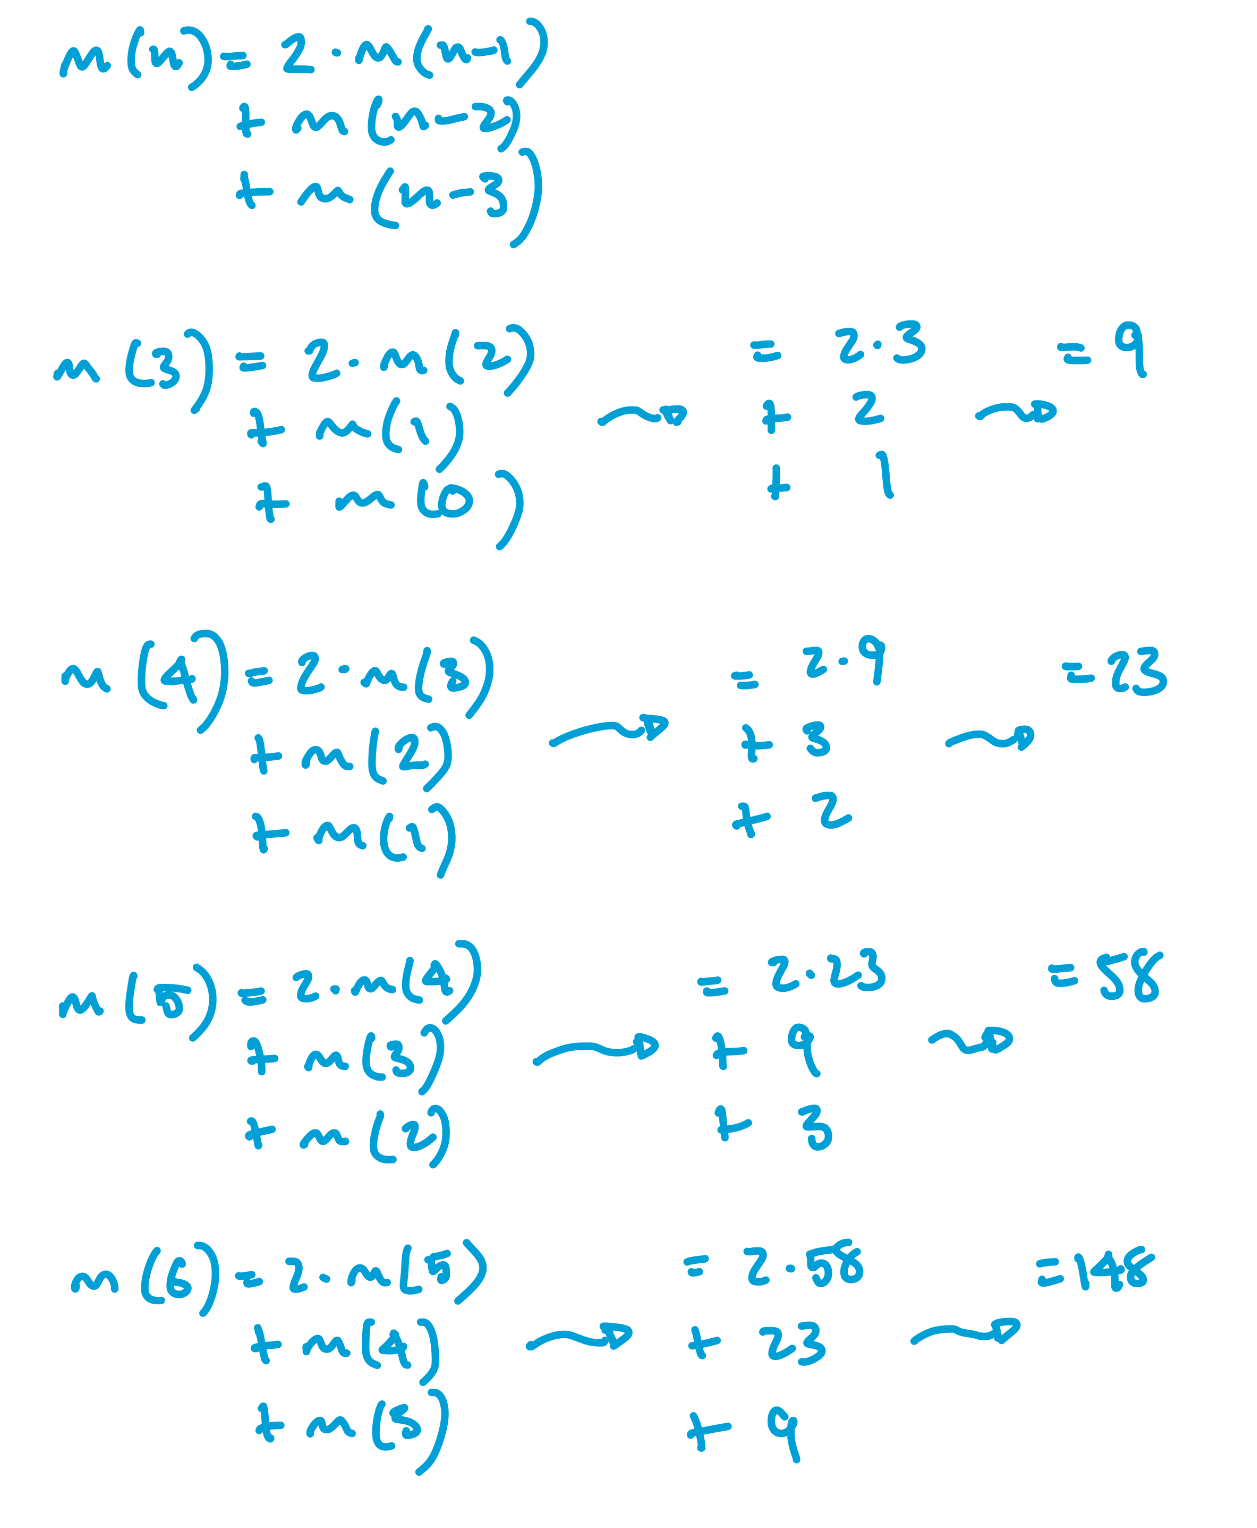
\includegraphics[width=0.8\textwidth]{table_working.jpeg}

\subsection{Implement}
I implemented a non-dynamic programming solution as well as dynamic.  I find having both versions very helpful for debugging and understanding.
\begin{lstlisting}[language=java]
static int computeM(int n){
  if (n == 0){
      return 1;
  } else if (n == 1){
      return 2;
  } else if (n == 2){
      return 3;
  } else {
      return 2*computeM(n-1) + computeM(n-2) + computeM(n-3);
  }
}

static int computeM_dynamic(int n){
  int[] memo = new int[Math.max(3,n+1)];
  memo[0] = 1;
  memo[1] = 2;
  memo[2] = 3;
  for (int i = 3; i <=n; i++){
      memo[i] = 2*memo[i-1] + memo[i-2] + memo[i-3];
  }
  return memo[n];
}
\end{lstlisting}
Please note that my dynamic solution looks slightly different to ones you will find in the textbooks, mine is definitely better.

\subsection{Partial Lookup}
We only ever use the last three values, so we don't need to keep a full table.  This version is much more subtle though, quite a bit harder to understand.  However, once you do understand it you can use the template in lots of places.  Note that the order of the assignments inside the loop is important and easy to get wrong.  I think the variable names I chose didn't work out that well, what would you use instead that would make the code "flow" better?
\begin{lstlisting}[language=java]
static int computeM_partial_memo(int n){
  if (n == 0) return 1;
  if (n == 1) return 2;
  if (n == 2) return 3;
  int curr = -1;
  int currlessone = 3;
  int currlesstwo = 2;
  int currlessthr = 1;
  for (int i = 3; i <=n; i++){
      curr = 2*currlessone + currlesstwo + currlessthr;
      currlessthr = currlesstwo;
      currlesstwo = currlessone;
      currlessone = curr;
  }
  return curr;
}
\end{lstlisting}

\subsection{Tests}
This is one case where the test is short and sweet
\begin{lstlisting}[language=java]
@Test
public void testComputeM(){
  for(int i = 0; i < 23; i++){
    assertEquals("normal vs dynamic for " + String.valueOf(i),
                  computeM(i), 
                  computeM_dynamic(i));
    assertEquals("normal vs partial for " + String.valueOf(i),
                  computeM(i), 
                  computeM_partial_memo(i));
  }
}
\end{lstlisting}
I've made use of a JUnit feature you may not have seen before.  You can add a string to most assertions which will get printed if that assertion fails.  This can really help you track down which input is causing the problem.  You can also see that having the non-dynamic version makes my tests even better because I have a simpler version to test both the complex versions against.  Note that I can't go over \verb|i = 23| because $m(24)$ is too big to fit in an integer and I get an overflow into negative numbers.  I.e. my code does not work for $m > 23$.  To make it work I would need to use doubles, which will get me some way, but ultimately I would have to switch to a reference type for integers.  We will save that for another day.

\section{Divide and Conquer: Strategies}
The answer lies somewhere between $0$ and $x$, but we don't know where.  We do know that if we try any particular number $n$ and $n*n$ is \emph{above} $x$, then we no longer need to check any of the numbers above $n$.  If we choose the midpoint as $n$ each time we guess, we can half the search space on every loop.  When doing any such binary search, you need to be careful of a few things, but they are the same for every binary search:
\begin{enumerate}
\item Don't choose the actual midpoint as the next lower or upper bound, choose one past the midpoint.
\item When you are done, it is the top of the range that is the correct answer.  You can trace to validate this.
\end{enumerate}

Here is my trace of the algorithm for $x$ of $19$

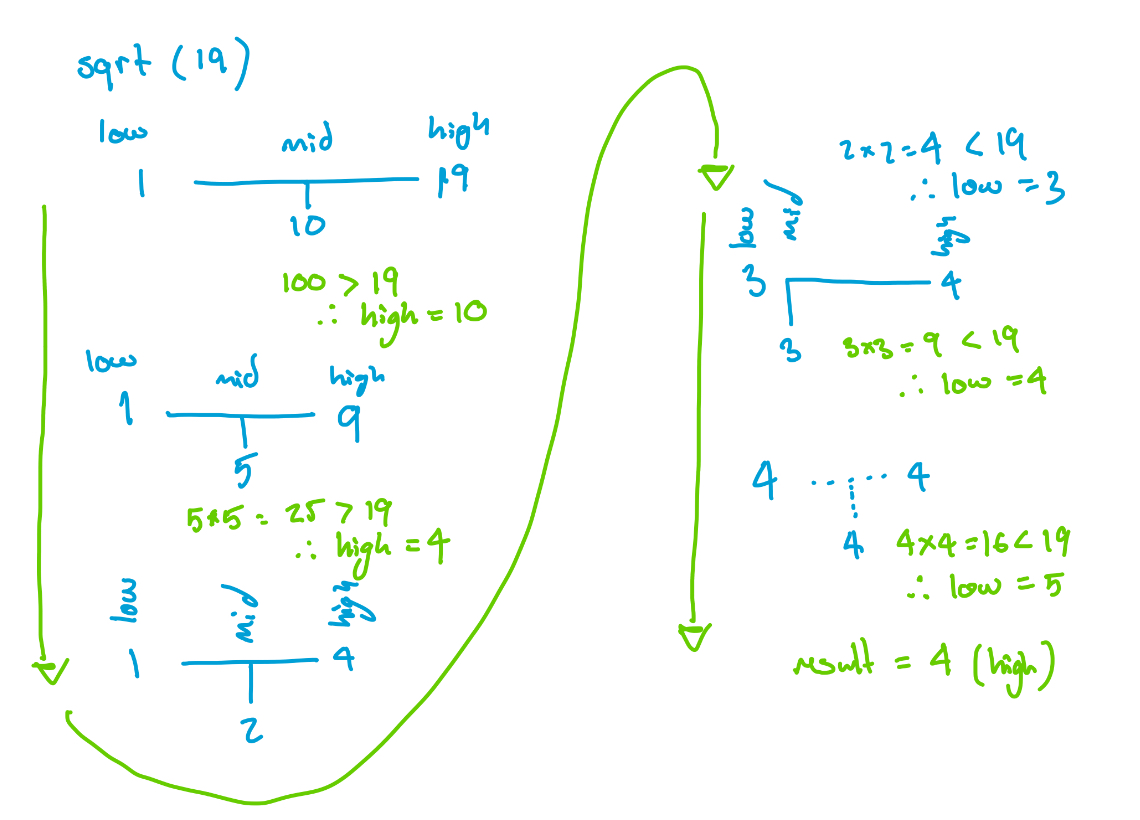
\includegraphics[width=\textwidth]{binary_search_trace.jpeg}
My solution is 

\begin{lstlisting}[language=java]
static int sqrt(int x){
      if (x <= 0) return 0;
      int low = 1;
      int high = x;
      while (low <= high){
          int mid = low + (high - low)/2;
          if (mid * mid == x) return mid;
          if (mid * mid < x)  low  = mid + 1;
          if (mid * mid > x)  high = mid - 1;
      }
      return high;
  }
\end{lstlisting}

\subsection{Big Oh}
I compute Big-Oh by:
\begin{enumerate}
\item Writing out the \emph{time function}. I get this by inspecting the code.  In this case I see that searching on $n$ causes either a) a result immediatly or b) a search on $n/2$ giving $T(n) = 3 + T(n/2)$
\item I've then got to get the "closed form"  of this.  I could go back to my maths and work this out, but the question included helpful table.  In this case I get $O(\log {n})$.  Below is  the on-paper working I did to get this solution
\item 
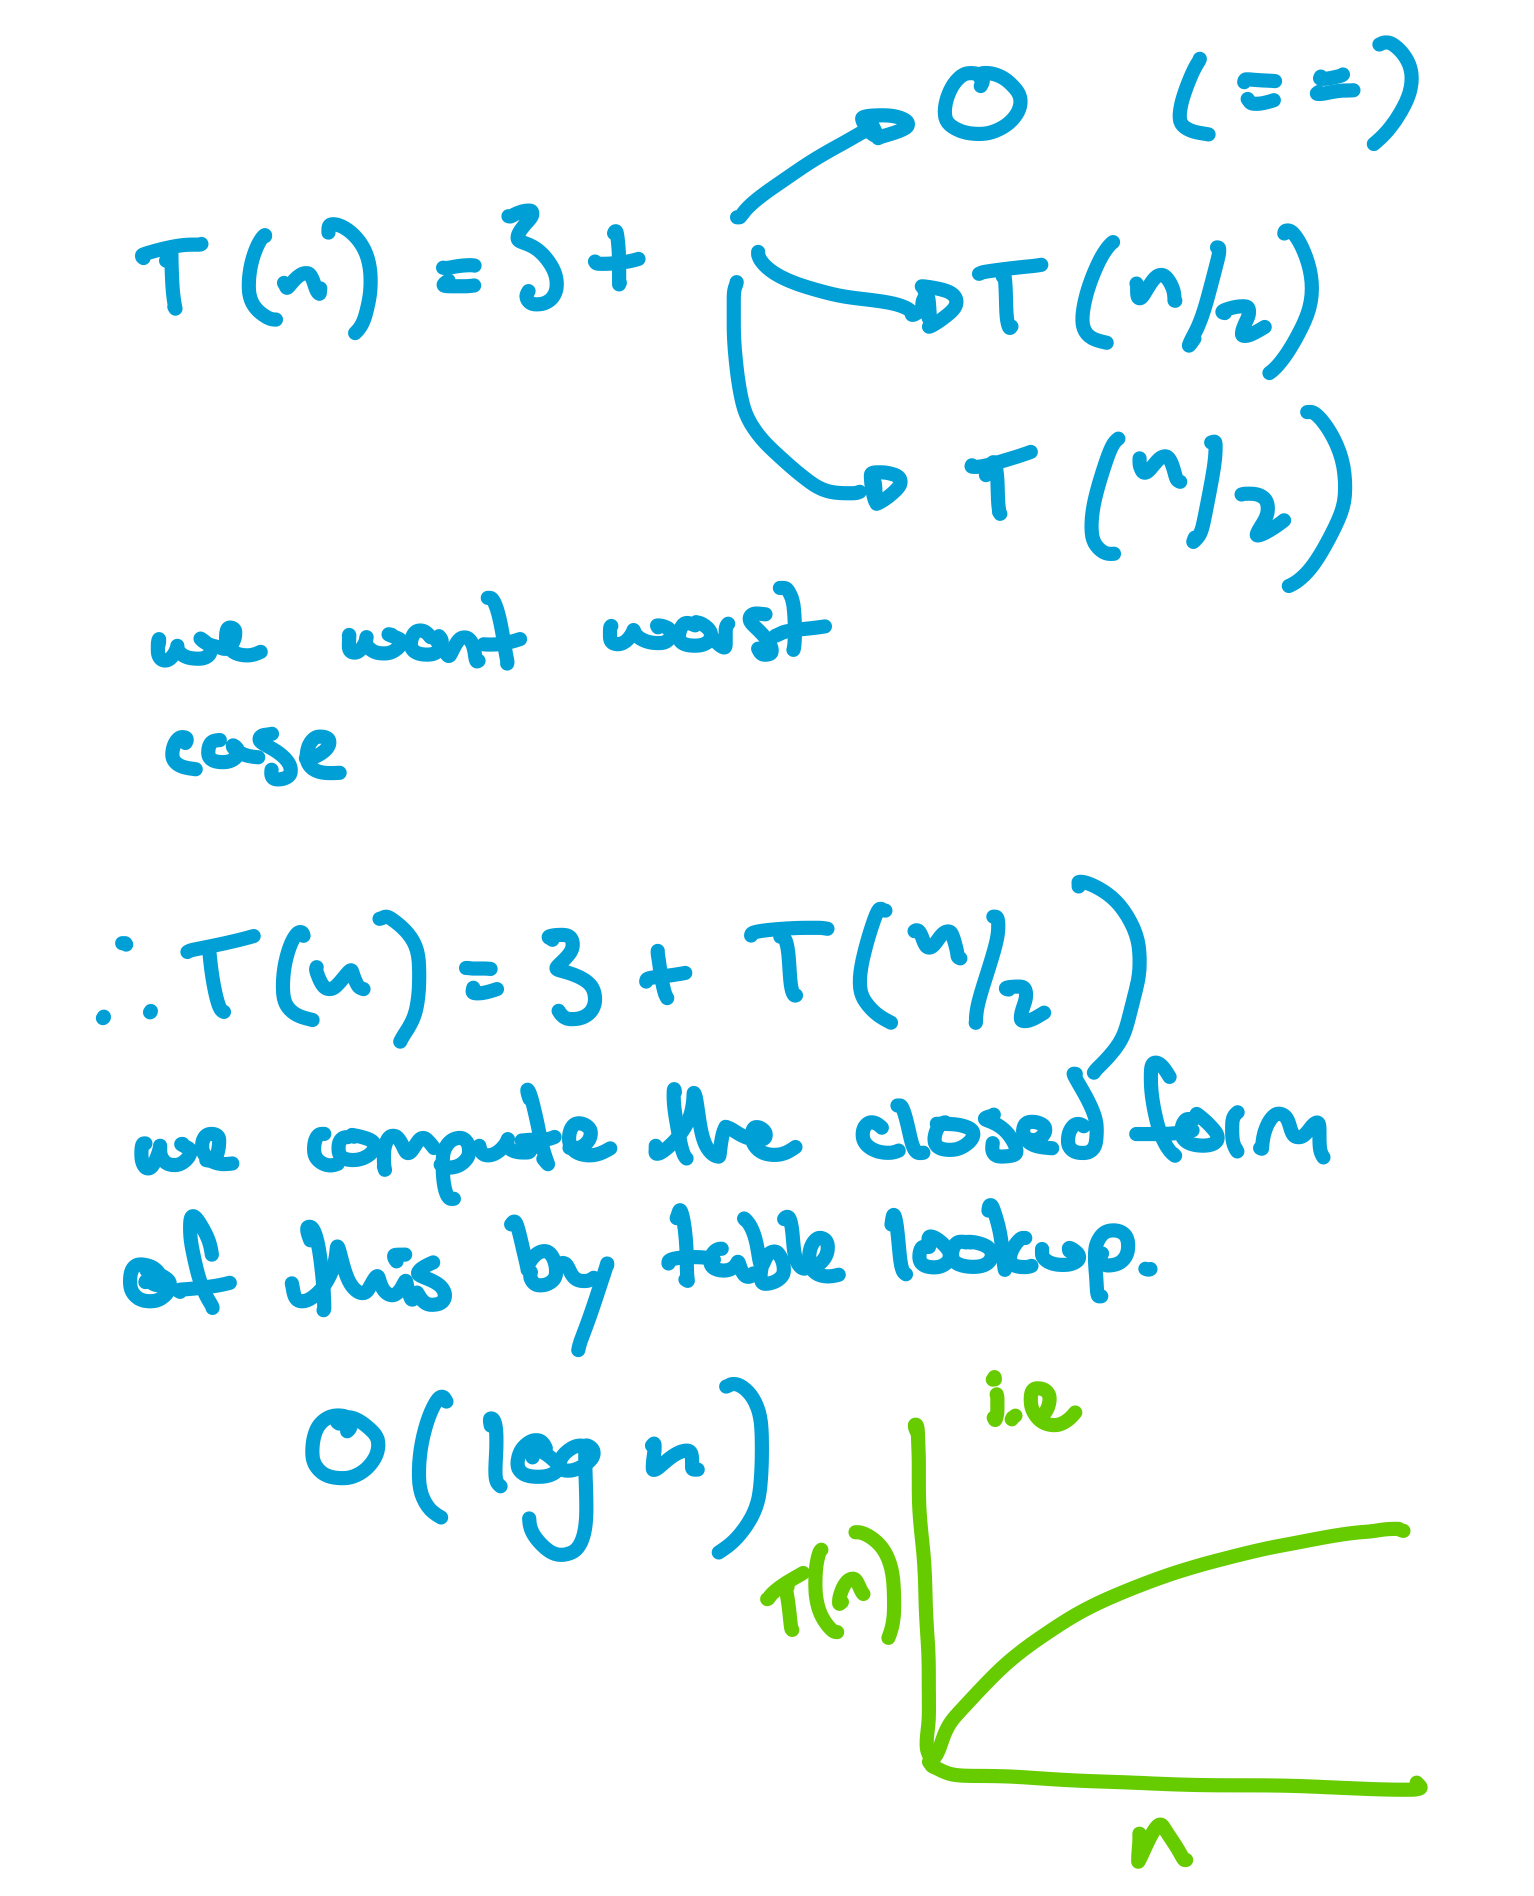
\includegraphics[width=0.7\textwidth]{binary_search_bigoh_trace.jpeg}

\end{enumerate}

\section{Divide and Conquer: Fast Power}
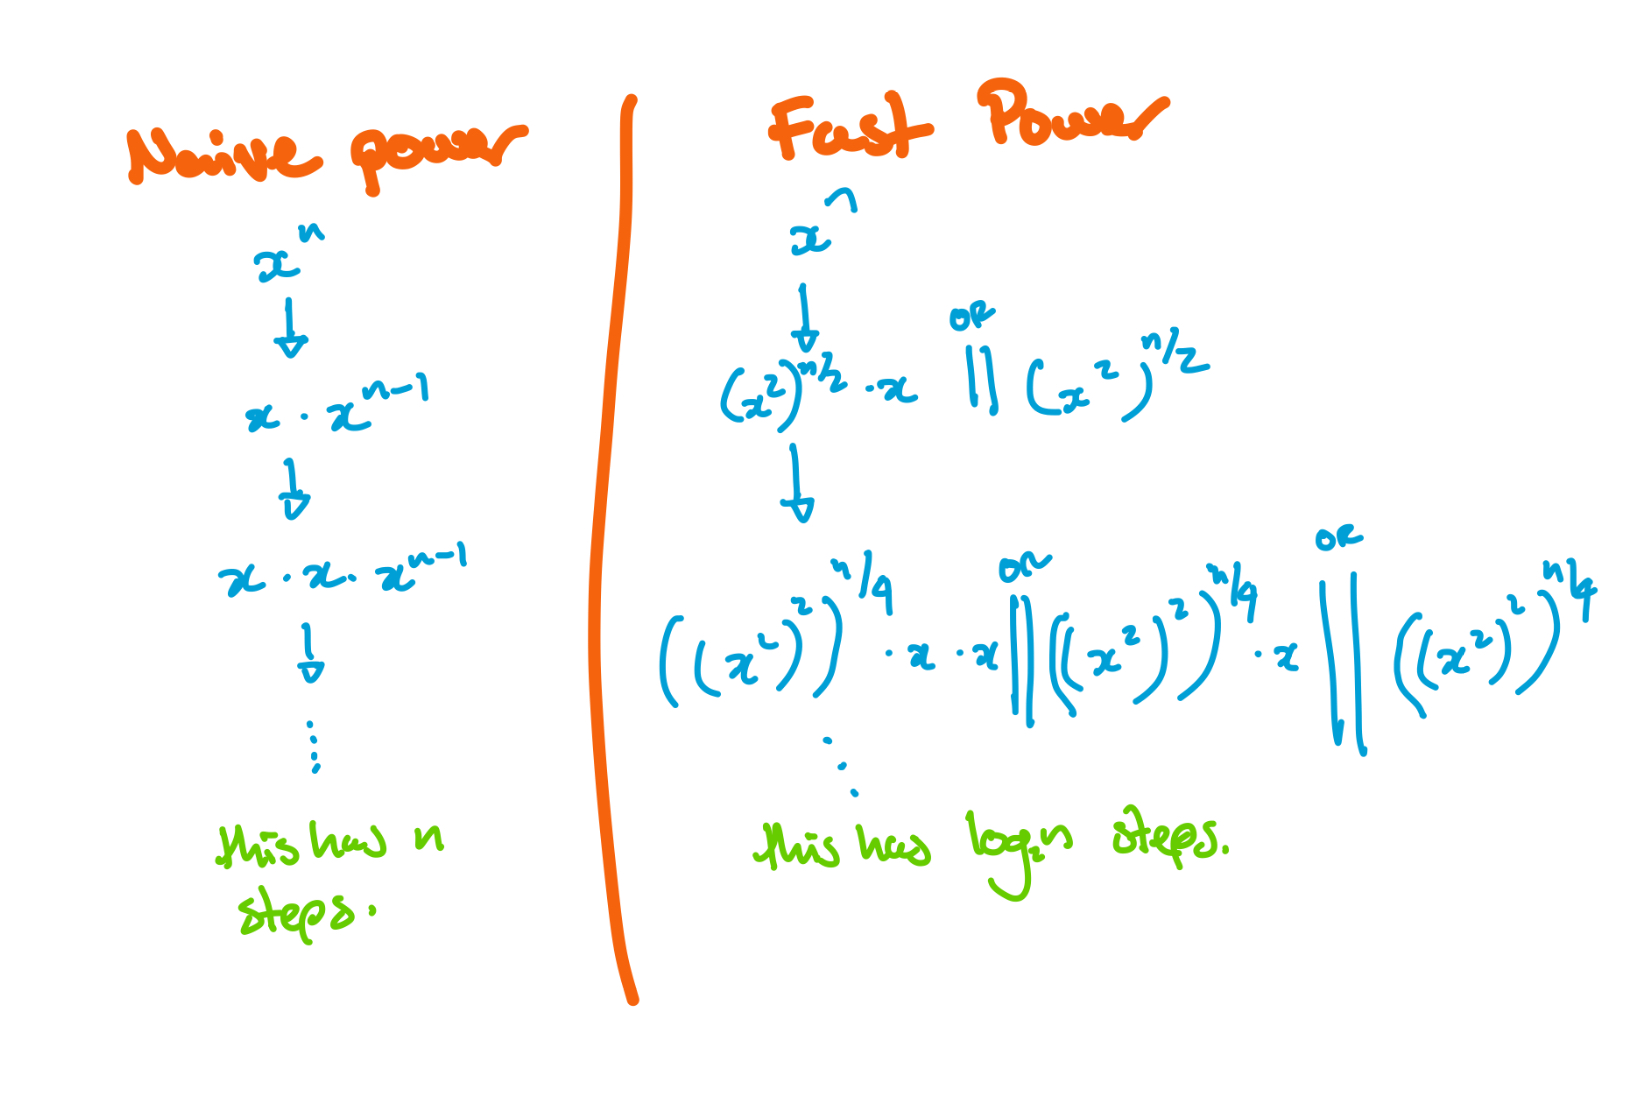
\includegraphics[width=\textwidth]{fast_power.jpeg}

\newpage\setcounter{section}{0}
\part*{Self Study}

\section{Recursion Iteration Iso: Binary Search}
In question \ref{sec:binary_search} we developed a binary search for the integer square root.  Take a look at your answer and decide if it is \emph{iterative} or \emph{recursive}.  Explain your reasoning.

\subsection{Alternative}
Whichever version you wrote, write the other.

\section{Divide and Conquer: Shift and Swift}
Suppose you are given an array $A$ of n sorted numbers that has been circularly shifted $k$ positions to the right. For example, 
\[
\{ 35, 42, 5, 15, 27, 29\}
\]
is a sorted array that has been circularly shifted $k = 2$ positions, while 
\[
\{27, 29, 35, 42, 5, 15\}
\]
has been shifted $k = 4$ positions.
      
\begin{enumerate}
    \item Suppose you know what k is. Give an $O(1)$ algorithm to find the largest number in $A$.
    \item  Suppose you do not know what $k$ is. Give an O(n) algorithm to find the largest number in $A$..
    \item Suppose you do not know what $k$ is. Give an $O(\log n)$ algorithm to find the largest number in $A$.
\end{enumerate}

\section{Dynamic Programming: Subsequence}
The \emph{longest common subsequence} problem is a classic example of dynamic programming which needs a two-dimensional table instead of an array like we used before.

\href{https://www.youtube.com/watch?v=ASoaQq66foQ}{This video}\footnote{\url{https://www.youtube.com/watch?v=ASoaQq66foQ}} is a great explanation of the longest common subsequence problem.  Watch it.

\subsection{Comparing the two traces}
\emph{Back to Back SWE} showed two traces, one which was the recursive solution, the second which used a dynamic programming table.

Trace the length of the longest common subsequence for the strings ``abcab" and ``abbca".  Perform \emph{both} types of traces from \emph{Back to Back SWE}.

\subsection{Big-Oh}
From your traces, try to work out the Big-Oh of each approach
\begin{hint}
This extended table might help

{\scriptsize
\begin{tabular}{llll}
    \hline 
    \textbf{description} & \textbf{iterative} & \textbf{recursive} & \textbf{Big Oh} \\
    \hline
    No loop & $T(n) = c_1$ &  & $O(1)$ \\
    Normal loop & $T(n) = c_1 + c_2*n$  & $T(n) = C_1 + C_2*T(n-1)$ & $O(n)$ \\
    Doubled Halving & & $T(n) = T(n/2) + T(n/2)$ & $O(n) $ \\
    Nested loop & $T(n) = n*n$ & $T(n) = c_1 + c_2*T(n-1)*T(n-1)$ & $O(n^2)$ \\
    Halving loop & $T(n) = n + n/2 + n/4 + \ldots + 1$ & $T(n) = C_1 + T(n/2) + T(n)$ & $O(\log{n})$ \\
    Work on both half & $T(n) = 2*(n + n/2 + \ldots + 1)$ & $T(n) = C_1 + T(n) + 2*T(n/2)$ & $O(n \log{n})$ \\
    Recursion on two  & & $T(n,m) = T(n-1, m) + T(n, m-1)$ & $O(2^{max(n,m)})$ \\
    Fill in a 2d table & $T(n) = n*m$ & $T(n,m) = n*T(m)$ & $O(n \times m)$ \\
\end{tabular}
}
  

\end{hint}
We won't ask you to implement longest common subsequence.  The naive solution is easy enough, but you need tables to do the dynamic one and you have not learned them yet.

\subsection{Dynamic Programming: Explore the Space}
\begin{note}
This question is an optional exploration which I find interesting and which really helped me understand Dynamic Programming but is not necessary for the course.
\end{note}

You have all the tools you need to implement the naive solution to the longest common subsequence.  I recommend you do this as an exercise.

If you then tried to implement the dynamic programming solution, you would feel like you are implementing a completely different algorithm.  However, the dynamic programming solution is actually just a tweaked version of the naive solution \emph{where each recursive call saves its return value to a table} so that, if it is called again, you can simply grab the value from the table instead of computing it all over again.

That's all dynamic programming is, just save each recursive call's answer in case it is needed again later.

You can implement this as a change to your naive solution using the \verb|Table| class provided in the code bundle.  That class lets you store an integer for each pair of strings, which is just what you would need.

Try out your two solutions on strings around length 20.  If your computer is close in speed to mine  you will find the naive solution taking up to a minute and the table solution taking less than a second!

As a last step, implement the dynamic programming solution we've been studying.  It is very neat, very small, and very fast.  Is it \emph{substantially} faster than the adjusted naive solution you came up with??

I've provided a \verb|StopWatch| class that might help you test speed accurately.

\section{Dynamic Programming: Practice, Practice, Practice}

\href{https://www.reddit.com/r/leetcode/comments/14o10jd/the_ultimate_dynamic_programming_roadmap/}{Reddit (yeah, reddit)}\footnote{\url{https://www.reddit.com/r/leetcode/comments/14o10jd/the_ultimate_dynamic_programming_roadmap/}} has a good list of dynamic programming problems from leetcode which are graded from simpler to hardest.   I recommend this as a source of practice problems.  I \emph{don't} recommend the linked video as the best explanation of the solutions.  You can find much better solutions out there.
 
\newpage\setcounter{section}{0}
\part*{Self Study Solutions}

\section{Recursion Iteration Iso: Binary Search}
My first one was iterative.  I know this because the body of the function has no call back to another instance of the same function.  Another clue is that there is a loop in my answer and that it covers all the possible answers in the loop.

\subsection{Alternative}
Here is the recursive solution.  Note that it needs a few extra parameters to work?  This happens sometimes with recursive functions.  We could study the general scheme to convert between them, but that belongs in another unit of study

\begin{lstlisting}
static int sqrt(int x, int low, int high){
  if (low > high) return high;
  int mid = low + (high - low)/2;
  if (mid * mid == x) return mid;
  if (mid * mid < x)  return sqrt(x, mid + 1, high);
  if (mid * mid > x)  return sqrt(x, low, high - 1);
  return high; // not really needed, unreachable code
} 
\end{lstlisting}

I personally much prefer the recursive one.  Putting parameters explicitly in the function signature really helps me to understand the code.

\section{Divide and Conquer: Swift and Shift}
The first two solutions should be obvious and are just to warm you up.  If you know $k$, the result is $A[k]$.  If you don't know $k$, just traverse from left to right and as soon as you see a decrease, you know the element you just passed is the biggest.  You don't even need to check the whole list (its still $O(n)$ though).

To get an $O(\log{n})$ solution when you don't know $k$, you \emph{must throw away half your data on each step}.  The only way to get \emph{any} $O(\log{n})$ solution is to throw away half the data on each setp.  We need two key insights to do that here:
\begin{enumerate}
\item If we see a pair of numbers next to each other and the right is bigger than the left, then the biggest number must be on the right hand side. We know this because, due to the shift, everything to the left is decreasing.
\item If we see a pair of numbers next to each other and the left is bigger than the right, then the biggest number must be on the left hand side.  We know this because, due to the shift, once we decrease, we can't get back up to the bigger element.
\end{enumerate}
This lets us do a binary search (with a twist) even though the array is not \emph{completely} sorted.  We get \emph{just enough} sorting to support the binary search.

\section{Dynamic Programming: Subsequence}
Here is my trace of the recursive solution.  I used red ink for the decision on the way down the recursive call and green for the result on the way up.  Where you see red dots there is more of the trace that I couldn't fit on a single page.  The point of a trace is to illuminate the algorithm to \emph{you} which is why I generally set a page as the maximum necessary size.

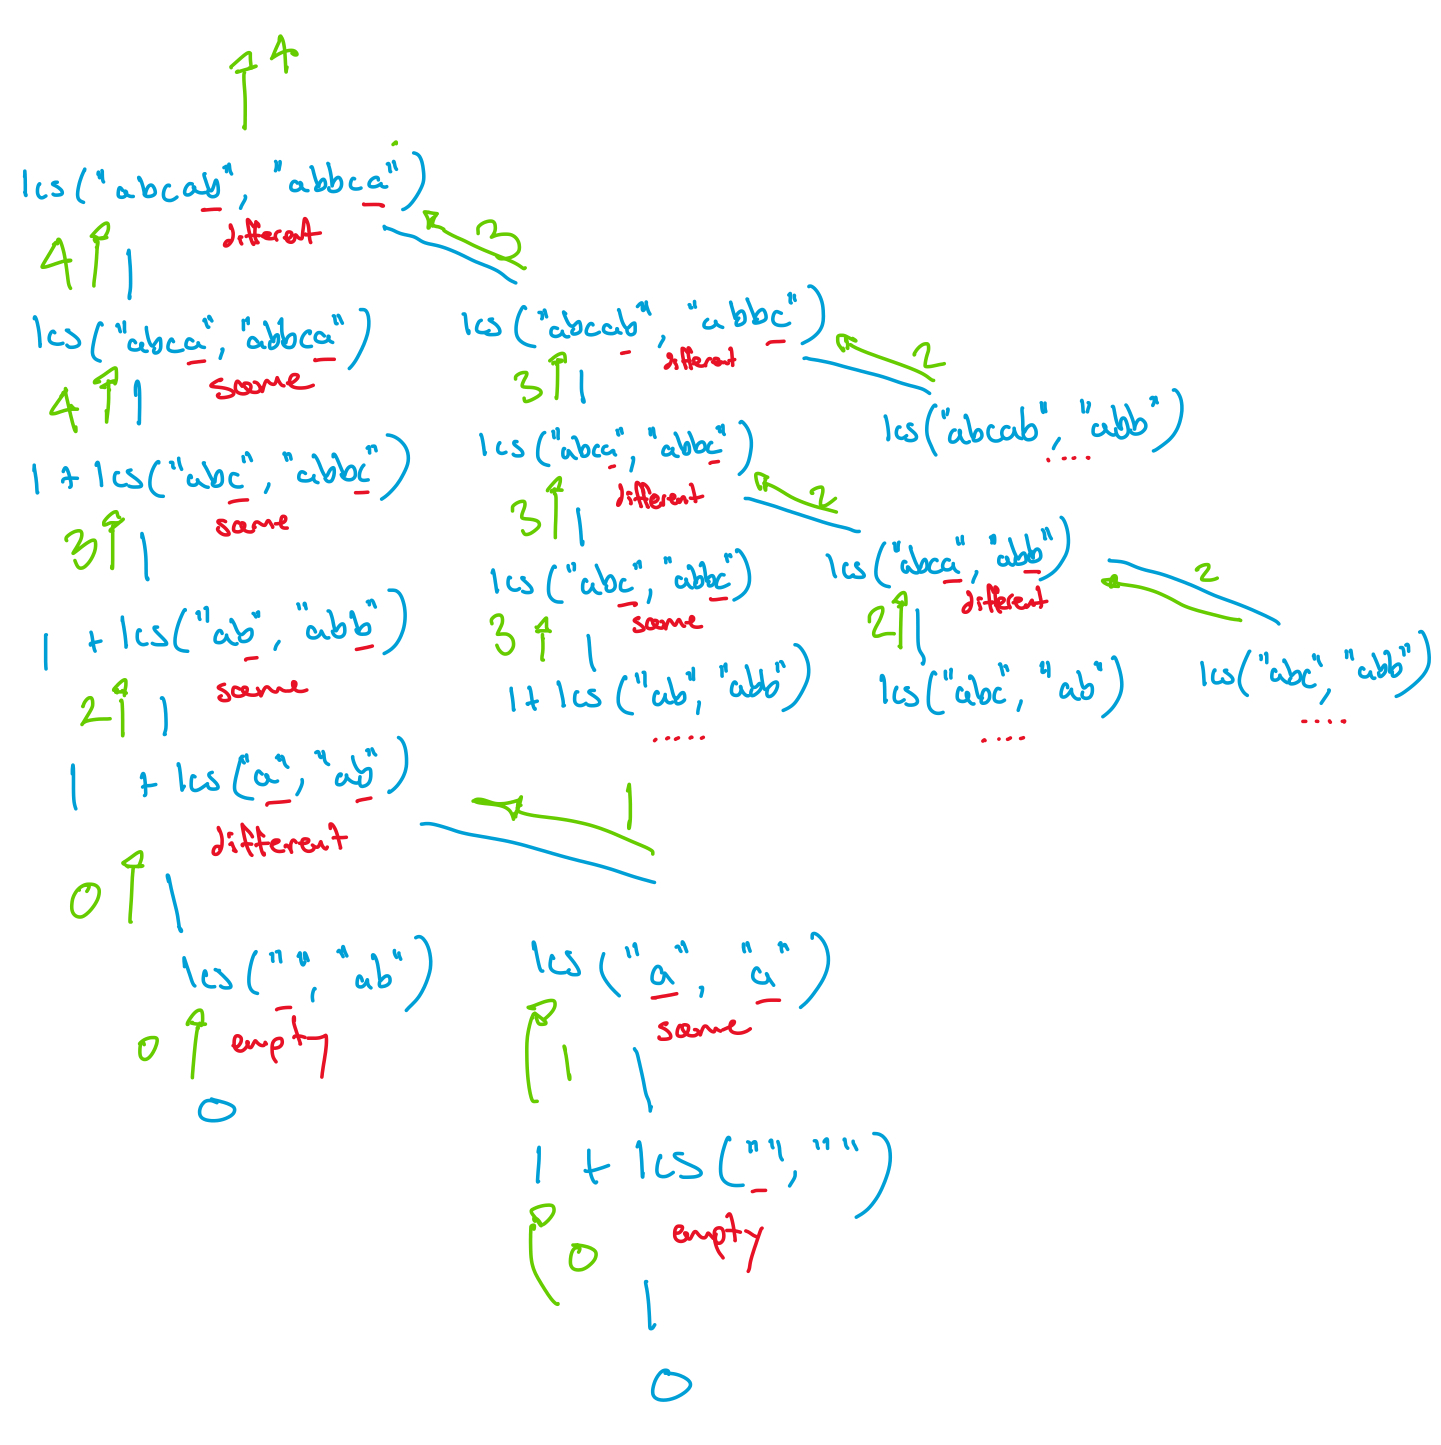
\includegraphics[width=\textwidth]{lcs_recursive.jpeg}

The Big-Oh of this solution is actually \emph{exponential}, which we haven't seen so far.  Lets think about the recursive time formula.  The length of both strings ($n$ and $m$) matter to the time.  On each call we might call one of two different things, call with both strings reduced by 1 or call with one string reduced by one:
$$
T(n,m) = T(n-1, m-1) \lor T(n-1, m) + T(n, m-1)
$$

If we assume we take the longest path each time we get 
$$
T(n,m) = T(n-1, m) + T(n, m-1)
$$
And our table tells us this is $O(2^{max(n,m)})$ which is very bad.  You can see from the trace how the exponential time complexity comes out.  The tree of recursive calls could \emph{double} at each level, which is what exponential means.

The trace for the dynamic solution is simply to fill in the table following the rule about when to add one and when to max the two around the cell.

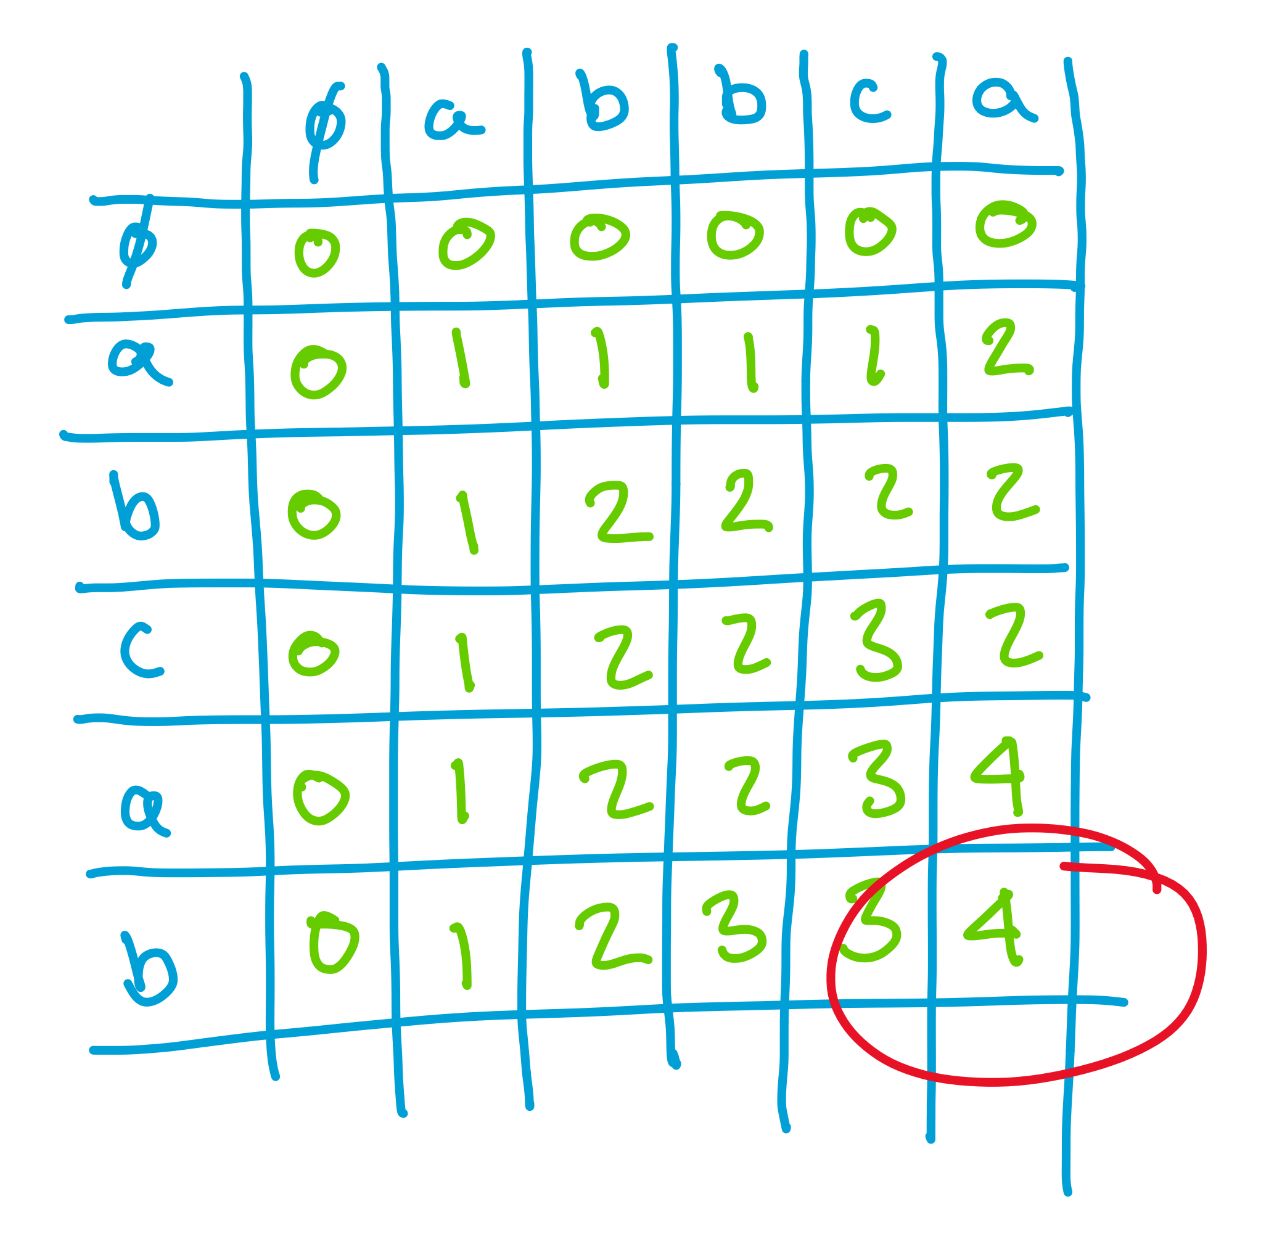
\includegraphics[width=0.7\textwidth]{lcs_dynamic.jpeg}

It is very easy to see the run time of this one is $O(n \times m)$.

\subsection{How are these two algorithms related}
Is one just a better solution, or are they actually related?  We've seen that \emph{remembering the sub-solutions in a recursive solution is what dynamic programming is} but it might not be obvious that is what is happening here.  Let's explore to find that connection.  Take a good look at this part of the recursive solution

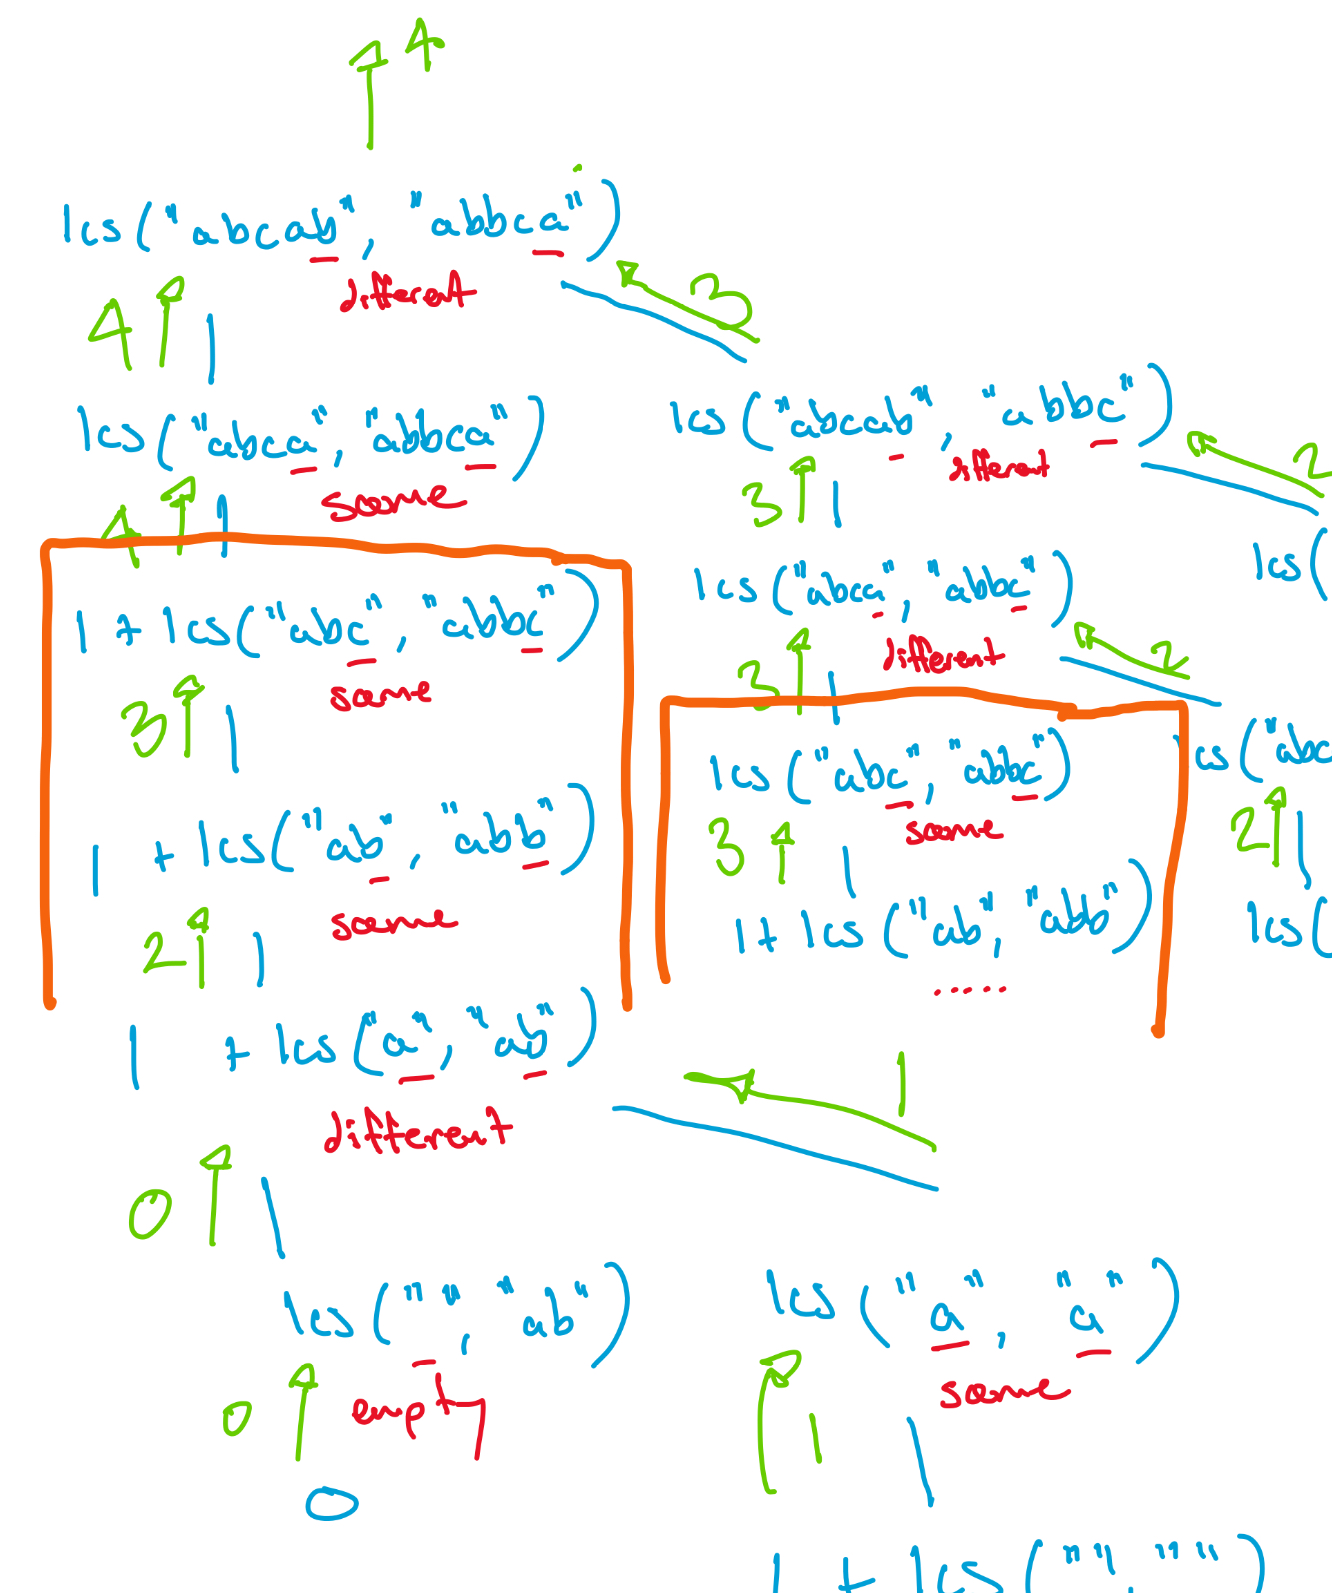
\includegraphics[width=0.7\textwidth]{lcs_recursive_close.jpeg}

The two orange regions are doing the exact same computation!  That is wasted effort.  When you have two parameters, you need a 2D table to store all those partial answers.  If you were to start from the recursive solution and just save the subparts then convert to an iterative solution, you will get the algorithm we've been using for the table.  It's just that when people teach it, then tend not to spend all that time on \emph{deriving} the dynamic solution, which is a shame.

\subsection{Dynamic Programming: Explore the Space}
My naive solution is
\begin{lstlisting}[language=java]
public static int naive(String a, String b){
    if (a.isEmpty() || b.isEmpty()){
        return 0;
    } else if (a.charAt(a.length()-1) == b.charAt(b.length()-1)){
        return 1 + naive(a.substring(0,a.length()-1), b.substring(0,b.length()-1));
    } else {
        return Math.max(
            naive(a.substring(0, a.length()-1),b),
            naive(a, b.substring(0, b.length()-1))
        );
    }
}
\end{lstlisting}

I got the optimised table solution by doing just two things:
\begin{enumerate}
\item Look up the table at the start of the recursive call to see if this pairing has already been computed.
\item Save values we compute to the table just before returning them.
\end{enumerate}
Otherwise the code is just the same.
\begin{lstlisting}[language=java]
static Table memoTable = new Table();
public static int memo(String a, String b){
    if (memoTable.get(a,b) >= 0) return memoTable.get(a,b);
    else{
        if (a.isEmpty() || b.isEmpty()){
            memoTable.add(a,b, 0);
            return 0;
        } else if (a.charAt(a.length()-1) == b.charAt(b.length()-1)){
            int ret = 1 + memo(a.substring(0,a.length()-1), b.substring(0,b.length()-1));
            memoTable.add(a,b,ret);
            return ret;
        } else {
            int ret =  Math.max(
                memo(a.substring(0, a.length()-1),b),
                memo(a, b.substring(0, b.length()-1))
            );
            memoTable.add(a,b,ret);
            return ret;
        }
    }
} 
\end{lstlisting}
It is as simple as this to get a dynamic programming solution and this solution has the same Big-Oh as the solution we've been working to.  It is slower overall, but has the same Big-Oh.

For completeness, here is my extra-neat solution which matches the dynamic programming solutions we find on the web.
\begin{lstlisting}[language=java]
public static int dp(String a, String b){
  int[][] table = new int[a.length()][b.length()];
  for(int i = 0; i < a.length(); i++){
      for(int j = 0; j < b.length(); j++){
          if(a.charAt(i) == b.charAt(j)){
              table[i][j] = (i == 0 || j == 0) ? 1 : table[i-1][j-1] + 1;
          } else {
              table[i][j] = (i ==0 || j == 0)? 0: Math.max(table[i-1][j], table[i][j-1]);
          }
      }
  }
  return table[a.length()-1][b.length()-1];
} 
\end{lstlisting}
You can see why people really love this solution and present it in this way. It is so neat and so short and so easy to trace.  However, we are learning dynamic programming so there is much value for us in seeing how to get to this solution from the naive one.

\subsection{Dynamic Programming: Practice, Practice, Practice}

No solutions given, the web is awash with people explaining leetcode so you will find good solutions there.

% \newpage\setcounter{section}{0}
% \part*{An algorithmic journey: Self-Study Part Two}
% \begin{todo}
% Add the real world example of this (chip testing) and expand this out to be a kind of wrap-up of the whole section. Include the invariants helping us understand our solutions and the explanation of the dynamic solution, and the pointer to hash-maps for another solutions to come.
% \end{todo}
% An array $A[0...n-1]$ is said to have a \emph{majority element} if \underline{more} than half of its entries are the same.\footnote{An array can't have more than one majority element.
%   E.g. $[2, 2, 4, 2, 4, 4]$ does not have a majority element, because neither 2 nor 4
%   appears more than half the time.}
% Given an array, the task is to design an efficient algorithm to tell whether the array has a majority element, and, if so, to find that element. The elements of the array are not necessarily from some ordered domain like the integers, and so there can be no comparisons of the form ``is $A[i]$  bigger than $A[j]$?''.  However, you can answer questions of the form: ``is $A[i] = A[j]$?'' in constant time.

% \section{Come up with an algorithm to solve this problem}
% This will require some imagination.  Try and think up your own algorithm and write it out as pseudo-code.  \emph{If} you can't think of one, you might ask-the-internet.  If you do ask-the-internet you should check that what you found is accurate.

% \section{What did you get?}
% There are actually half-a-dozen algorithms for solving this problem.  To work out which one you found, work out the time complexity of your solution.  Look up this table to see what version you (probably) got

% \begin{tabular}{|l|l|}
%   \hline
%   $O(n)$ & hash map solution\\
%   $O(n^2)$ & brute force \\
%   $O(n \log{n})$ & dynamic algorithm \\
%   $O(\log{n})$ &  you might have sorted, which isn't allowed \\
%   \hline
% \end{tabular}

% Once you have an idea, look it up to see if your solution really is the type I've suggested

% \section{The Dynamic Solution}
% We will now investigate the dynamic algorithm that solves this problem in $O(n \log{n})$.  If you already came up with this version - well done!  You can jump to the next question.

% Consider splitting the array $A$ into two arrays $A_1$ and $A_2$ of half the size. If you know the 
% majority elements of $A_1, A_2$ and how many  there are (in the original array),  show how that helps you figure out the majority element of $A$.
 
% Using this, construct a Divide and Conquer algorithm for finding the majority. 

% \newpage\setcounter{section}{0}
% \part*{An algorithmic journey: Self-Study Part Two Solution}
% \section{Come up with an algorithm to solve this problem}
% I came up with the following.  Keep a table with one entry for each value you find in the array (you can add new entries as you come across new values).  Loop through the array from start to finish and for each element you find, add 1 to its entry in the table.  At the end of the loop, the table row with the highest number is your candidate.  Check the candidate frequency is more than half the array length then report it as the answer.

% \section{What did you get}
% My solution is $O(n)$ so I must have found the "hash table" algorithm.  Indeed I did and I would not expect many of you to get this solution since you haven't learnt hash tables yet!  But you will, and then this solution will be in your arsenal.

% More likely you got the "brute force" solution if you worked it out yourself.  Unless you were alert enough to realise we are studying dynamic algorithms at the moment and managed to find that solution.  It is not an easy solution to find though and you probably need the tips from the next question to find it.


% \begin{note}
% The majority element \emph{is not} the most common element. It has to be at least half the array to count!  This mistake catches out so many students studying this example.
% \end{note}
% Consider the two arrays
% \begin{lstlisting}
%   int[] a = {1,1,1,2,2};
%   int[] b = {2,2,2,3,3};
% \end{lstlisting}
% The majority element of \verb|a| is 1 (three time) and the majority element of \verb|b| is 2 (three times).  If the two arrays are combined
% \begin{lstlisting}
%   int [] ab = {1,1,1,2,2,2,2,2,3,3}
% \end{lstlisting}
% has major element 2.  This example might convince us that the major element of the full array must have been one of the majority elements of the split arrays.  Try to adjust them a little so 2 is not the majority element of its subarray but is the majority element of the combined array.  You can't do it.  As soon as it gets below majority for the sub-array, there are not enough of them to make it majority of the combined array.  It's not that easy to see, but the majority element of a combined array can only be either the majority array of the left half, the majority element of the right half, or nothing.

% Let's run a few more combinations to really convince you.  Since we will split by half (we should know by now that is a smart move), the subarrays can't differ by more than one.

% \begin{tabular}{ccccc}
% \\
% $[1,2,3,4]$ & + & $[4,4,4]$ & $\rightarrow$ & $[1,2,3,4,4,4,4]$ \\
% $\phi$ & & 4 & & 4 \\ \\ \hline \\
% $[1,1,1,1]$ & + & $[4,4,4]$ & $\rightarrow$ & $[1,1,1,1,4,4,4]$ \\
% 1 & & 4 & & 1 \\ \\ \hline \\
% $[1,1,1,4]$ & + & $[4,4,4]$ & $\rightarrow$ & $[1,1,1,4,4,4,4]$ \\
% 1 & & 4 & & 4 \\ \\ \hline \\
% $[1,1,1,2]$ & + & $[4,4,4,2,2]$ & $\rightarrow$ & $[1,1,1,2,4,4,4,2,2]$ \\
% 1 & & 4 & & $\phi$  \\ \\ \hline \\
% \end{tabular}

% Alright, I am convinced
% \begin{quote}
% The majority element of the whole array must be a majority element of at least one of the subarrays if I split it in half
% \end{quote}

% The examples above also show that \emph{there is not enough information in the subarrays to help you choose which of the sub-majority elements to choose}.  The only way to choose is to count how many there are in the 
% So, lets re-do the example, knowing the complete array will be 

% TODO: Complete
\end{document}